%%%% NeurReps 2026 — Extended Abstract Track (non-archival, double-blind) %%%%
\documentclass[mlabstract,onecolumn]{jmlr}

% Watermark — remove for camera-ready
\usepackage[hpos=300px,vpos=70px]{draftwatermark}
\SetWatermarkText{}
\SetWatermarkScale{1}
\SetWatermarkAngle{0}

% amsmath, amssymb, natbib, graphicx, url, algorithm2e are auto-loaded
\usepackage{booktabs}

\def\R{\mathbb{R}}
\newcommand{\Ham}{H}
\newcommand{\flip}{R}

\jmlrvolume{}
\jmlryear{2026}
\jmlrworkshop{Symmetry and Geometry in Neural Representations}

\title[Flow-Map Surrogates for HMC]{Learned Flow Maps as Hamiltonian Monte Carlo
Proposals, and the Symmetry They Require}

% Authors omitted for double-blind review.

\begin{document}

\maketitle

\begin{abstract}
Surrogate Hamiltonian Monte Carlo learns a cheap stand-in for an expensive
log-density gradient during warm-up. Every such method we are aware of learns a
\emph{vector field} --- a gradient, or an energy that is differentiated --- and
places it inside a symplectic integrator, so advancing $L$ leapfrog steps costs
$L$ sequential network evaluations. We propose learning the \emph{flow map}
instead, which costs one evaluation regardless of $L$. Symplectic neural
networks are the natural function class, and to our knowledge they have not
previously been used as MCMC proposals; the surrogate literature learns fields
inside integrators, and the symplectic-network literature predicts dynamics.
Making the substitution work requires more than symplecticity. A Hamiltonian
flow carries two structures --- it preserves the symplectic form, and it is
time-reversal symmetric --- and a Metropolis correction consumes the second, in
the form of an involution. Symplectic networks supply the first by architecture
and the second not at all, missing it by $\mathcal{O}(10^{-1})$, so they are not
admissible proposals as they stand. Composing the network with its
momentum-conjugate inverse restores the missing symmetry exactly, as an
algebraic identity in the weights and at no cost in parameters; this is the
construction of \citet{valperga2022reversible}, which we transfer from dynamics
prediction to sampling and instantiate with closed-form inverses for the LA- and
G-SympNet layers. We also find that the conventional all-pairs training set is
not merely wasteful but harmful --- supervising only the single time offset the
sampler queries is $1275\times$ cheaper at $L=50$ and fits better. On
Gaussian-process hyperparameter inference at the configuration of
\citet{Li_2019}, the resulting sampler attains $3.7\times$ the effective samples
per second of exact HMC, while every integrator-based surrogate we test is
\emph{slower} than exact HMC. We report one cautionary result throughout: an
unsymmetrized network posts a competitive $142$ ESS/s at a reversibility error
of $5\times10^{-4}$, so effective sample size alone cannot certify a learned
proposal.
\end{abstract}

\begin{keywords}
symplectic neural networks, Hamiltonian Monte Carlo, time-reversal symmetry,
structure-preserving architectures, surrogate models
\end{keywords}

\section{Learning the flow map instead of the field}

Hamiltonian Monte Carlo \citep{Brooks_2011} proposes states by integrating
Hamiltonian dynamics and corrects the discretisation error with a Metropolis
step. When the target's gradient is expensive, surrogate methods learn a cheap
stand-in during warm-up: a gradient \citep{Li_2019}, or a Hamiltonian that is
differentiated \citep{DHULIPALA2023112425}. In every such method the learned
object is a \emph{vector field} placed inside a symplectic integrator. That
arrangement is why they remain asymptotically exact --- an inaccurate network
lowers the acceptance rate but cannot bias the chain --- and it also fixes their
cost: advancing $L$ leapfrog steps requires $L$ sequential network evaluations.

We propose learning the flow map $\hat\phi(z,\tau)$ directly. Because the
elapsed time is an input, a proposal costs one evaluation regardless of $L$, and
the saving grows with trajectory length --- the regime adaptive schemes such as
NUTS \citep{hoffman2011nouturn} and ChEES \citep{hoffman2021adaptive} push
towards. Symplectic neural networks \citep[SympNets;][]{jin2020sympnets} are the
natural function class, sitting in a broader effort to learn Hamiltonian
dynamics with architectural constraints
\citep{greydanus2019hamiltonian,chen2019neural}.

To our knowledge this bridge has not been crossed. The surrogate-HMC literature
learns fields inside integrators; the symplectic-network literature predicts
dynamics and does not treat sampling. The requirement we identify below is
therefore a design constraint on a construction we are proposing, not a
correction to published work.

\paragraph{Contributions.}
\begin{itemize}
    \item We propose learned symplectic flow maps as HMC surrogates, motivated
    by an $\mathcal{O}(1)$ rather than $\mathcal{O}(L)$ per-proposal cost.
    \item We identify what the substitution requires. Replacing the integrator
    forfeits the correctness it was supplying: a SympNet satisfies volume
    preservation but violates involutivity by $\mathcal{O}(10^{-1})$, and no
    amount of training data repairs it (Table~\ref{tab:validity}). The symmetrised
    map of \citet{valperga2022reversible} restores it exactly, and we give
    closed-form inverses for the LA- and G-SympNet layers so the construction
    is exact rather than approximate.
    \item We find the conventional all-pairs training set actively harmful:
    supervising only the offset the sampler queries is $1275\times$ cheaper at
    $L=50$ and yields \emph{higher} effective sample size (Appendix~\ref{app:pairs}).
    \item Empirically the symmetrised flow map attains $3.7\times$ the ESS/s of
    exact HMC on GP hyperparameter inference, where every integrator-based
    surrogate is slower than exact HMC (Figure~\ref{fig:results}).
\end{itemize}

\section{What a deterministic proposal requires}

Let $\pi(z) \propto e^{-\Ham(z)}$ on $\R^{2D}$ with $\Ham \circ \flip = \Ham$,
where $\flip(q,p) = (q,-p)$. A Metropolis--Hastings scheme proposing $z' = T(z)$
deterministically and accepting with probability
$\min\{1, e^{\Ham(z) - \Ham(Tz)}\}$ leaves $\pi$ invariant provided
\begin{align}
    \text{(V)} \quad & |\det \nabla T(z)| = 1, \label{eq:vol}\\
    \text{(I)} \quad & (\flip \circ T) \circ (\flip \circ T) = \mathrm{Id},
    \label{eq:inv}
\end{align}
volume preservation and involutivity of $\flip \circ T$
\citep{Green1995,Tierney1998}. Leapfrog integration of any position-dependent
force satisfies both identically --- which is exactly what a flow map gives up.
That neural proposals must be engineered to satisfy these conditions is
established \citep{song2017nice,levy2018generalizing}, and
\citet{spanbauer2020involutive} give a general construction from
volume-preserving involutions.

A SympNet composes layers that update either $q$ or $p$ using a function of the
other, unmodified half of the state; for the gradient module in ``up'' mode,
$(q,p) \mapsto (q,\; p + \tau\, K^{\!\top} a\, \sigma(Kq + b))$. Each layer has
unit-determinant Jacobian, so \eqref{eq:vol} holds for any weights.
Condition~\eqref{eq:inv} concerns how the map interacts with $\flip$, and no
layer constrains it.

\paragraph{Closed-form inverses.} The shear structure that makes SympNets
symplectic also makes them exactly invertible: in an ``up'' layer the position
passes through untouched, so the increment added to $p$ can be recomputed from
the output and subtracted. Composing layer inverses in reverse order gives
$\Phi_t^{-1}$ exactly; we measure
$\|\Phi_t^{-1}\Phi_t z - z\|_\infty \approx 10^{-15}$.
\citet{valperga2022reversible} build their reversible architecture from
H\'enon maps and coupling layers; the SympNet modules admit the same treatment,
which lets the construction apply to networks already in use.

\paragraph{The symmetrised map.} Following \citet{valperga2022reversible},
\begin{equation}
    \Psi_t \;:=\; \flip \circ \Phi_{t/2}^{-1} \circ \flip \circ \Phi_{t/2}.
    \label{eq:psi}
\end{equation}

\begin{proposition}
\label{prop:involution}
If $\Phi_{t/2}$ is invertible then $\Psi_t$ satisfies \eqref{eq:inv}; if it is
additionally symplectic then $\Psi_t$ satisfies \eqref{eq:vol}. The chain with
proposal $\Psi_t$ therefore leaves $\pi$ invariant for arbitrary weights.
Moreover if $\Phi_s$ is the exact flow of a momentum-even Hamiltonian then
$\Psi_t = \Phi_t$, so the construction does not perturb an exact model.
\end{proposition}

Proofs are in Appendix~\ref{app:proof}. Two consequences are worth stating. The map
costs two network evaluations and \emph{no additional parameters}, so a $\Psi$
built from an $n$-block network has the effective depth of a plain $2n$-block
network with half the parameters --- comparisons must control for effective
depth, not block count. And the property survives composition: if
$\flip \Psi \flip = \Psi^{-1}$ then $(\flip \Psi^{k})^2 = \mathrm{Id}$ for
every $k$, so multi-step trajectories remain valid proposals.

\paragraph{What the sampler queries.} Flow maps are conventionally trained on
all pairs $(x_i,x_j)$, $i<j$, from each warm-up trajectory, giving
$\mathcal{O}(L^2)$ examples. But the sampler evaluates $\hat\phi$ at exactly one
offset, $\tau = L\epsilon$. With finite capacity, fitting times the sampler
never queries takes capacity from the one it does; Appendix~\ref{app:pairs} shows this
costs both compute and accuracy.

\section{Results}

Models are trained on warm-up trajectories from exact HMC and used as proposals,
corrected with the exact Hamiltonian, under a shared optimisation protocol so
comparisons reflect architecture rather than tuning. Timings use an isolated GPU.

Table~\ref{tab:validity} evaluates \eqref{eq:vol} and \eqref{eq:inv} at random
initialisation, emphasising that these are properties of the construction rather
than of training. Figure~\ref{fig:results} reports GP hyperparameter inference at the
configuration of \citet{Li_2019} ($n=500$, Mat\'ern $\nu=3/2$, $\epsilon=0.05$,
$L=20$, $10^4$ samples), where each gradient costs an $\mathcal{O}(n^3)$
Cholesky. The symmetrised flow map reaches $177$ ESS/s against exact HMC's
$48$; the gain is wall-clock rather than sample quality, since HMC attains
higher raw ESS ($18\,634$ versus $11\,609$) in $6\times$ the time. Every
integrator-based surrogate is slower than exact HMC ($0.41$--$0.83\times$). The
advantage grows with $L$, and the integrator-based surrogate degrades sharply as
$L$ grows because it applies its learned field $L$ times and compounds error at
each step, whereas the flow map applies once.

\begin{table}[t]
\centering
\caption{Validity conditions at random initialisation ($D=2$, $L=5$,
$\epsilon=0.1$, double precision). Volume preservation is
$\max|{\det \nabla T}|-1$; involutivity is $\max\|(\flip T)^2 z - z\|_\infty$.}
\label{tab:validity}
\begin{tabular}{lccc}
\toprule
proposal map & $|\det \nabla T| - 1$ & involution error & valid \\
\midrule
Exact leapfrog (HMC)                  & $2\cdot10^{-16}$ & $3\cdot10^{-16}$ & yes \\
Learned field $+$ leapfrog            & $8\cdot10^{-16}$ & $9\cdot10^{-16}$ & yes \\
\midrule
LA-SympNet (plain)                    & $1\cdot10^{-15}$ & $2.4\cdot10^{-1}$ & \textbf{no} \\
G-SympNet (plain)                     & $7\cdot10^{-16}$ & $1.2\cdot10^{-1}$ & \textbf{no} \\
LA-SympNet (symmetrised)              & $2\cdot10^{-15}$ & $4\cdot10^{-16}$ & yes \\
G-SympNet (symmetrised)               & $7\cdot10^{-16}$ & $1\cdot10^{-16}$ & yes \\
\bottomrule
\end{tabular}
\end{table}

\begin{figure}[t]
\centering
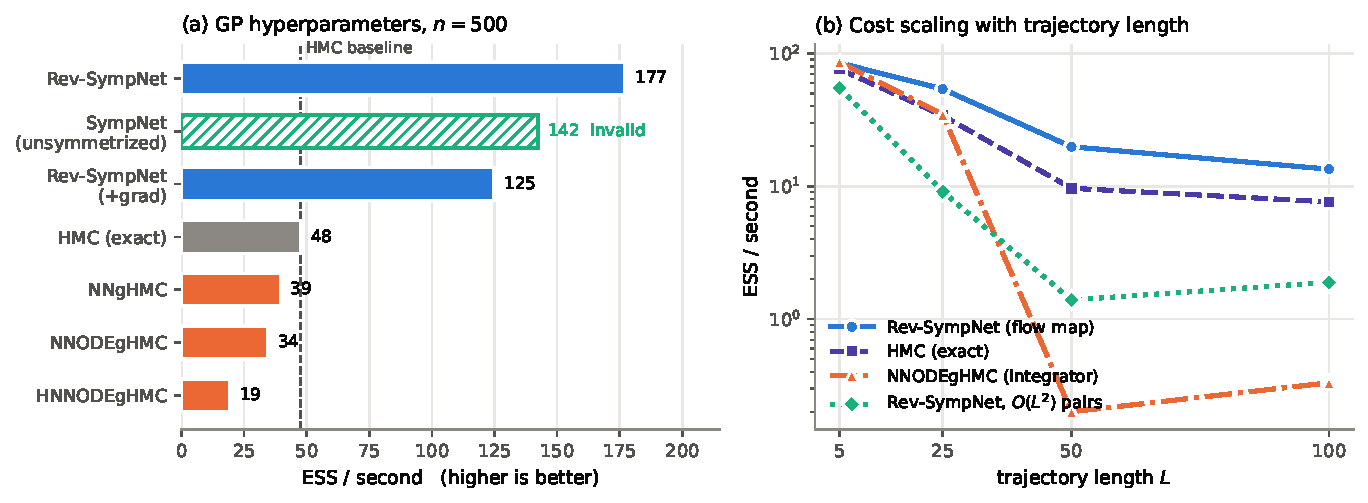
\includegraphics[width=\textwidth]{results.pdf}
\caption{(a) GP hyperparameter inference; best value over training budgets. The
symmetrised flow map attains $3.7\times$ the ESS/s of exact HMC, while every
integrator-based surrogate is slower than exact HMC. The unsymmetrised network
(hatched) posts a competitive number at a reversibility error of
$5\times10^{-4}$ and is not a valid sampler. (b) ESS/s against trajectory
length: the flow map's advantage grows with $L$, the integrator-based surrogate
collapses, and training on $\mathcal{O}(L^2)$ pairs erases the gain.}
\label{fig:results}
\end{figure}

\paragraph{Effective sample size does not certify a proposal.} In
Figure~\ref{fig:results} the unsymmetrised network attains $142$ ESS/s, which would
read as a $3\times$ improvement over exact HMC, at a reversibility error of
$5\times10^{-4}$. A map with a large involution defect can produce weakly
autocorrelated paths while targeting the wrong distribution; ESS measures
autocorrelation, not correctness. We note this because the artefact is easy to
mistake for a result, and we recommend reporting a structural diagnostic, or a
two-sample distance against a reference chain, alongside any ESS for a learned
proposal.

\section{Limitations}

Our targets are low-dimensional (two to thirty parameters). A flow map must
represent a map on the full $2D$-dimensional phase space, whereas
gradient-learning surrogates fit a field on the $D$-dimensional position space
alone, and we would expect that gap to widen with dimension. Our speedups are
measured on GPU, where a $500\times500$ Cholesky costs about $4$\,ms and the
gradient is not the dominant per-step cost; \citet{Li_2019} report $39.3\times$
for a gradient-learning surrogate on their hardware, which we do not reproduce
($0.83\times$) at matched $n$ and $L$. Our advantage comes from a different
mechanism --- collapsing $L$ sequential operations into one --- and the two
numbers are not comparable. Finally, supervising only the queried offset fixes
the trajectory length at training time; adaptive-length schemes would require
the $\mathcal{O}(L)$ construction, at a measurable cost in fit. Making
trajectory length adaptive for a flow map, where length carries no per-proposal
cost, is the natural next question.

Code for every experiment, together with the result files behind each reported
number, is included in the anonymized supplementary material.

\appendix

\section{Proof of Proposition~\ref{prop:involution}}
\label{app:proof}

Write $\Phi := \Phi_{t/2}$. Since $\flip^2 = \mathrm{Id}$,
$\flip \circ \Psi_t = \Phi^{-1} \circ \flip \circ \Phi$, a conjugation of the
involution $\flip$, hence an involution:
$(\flip \Psi_t)^2 = \Phi^{-1}\flip\,\Phi\,\Phi^{-1}\flip\,\Phi
= \Phi^{-1}\flip^2\Phi = \mathrm{Id}$, which is \eqref{eq:inv}. For
\eqref{eq:vol}, $\flip$ is anti-symplectic, so $\flip \Phi^{-1} \flip$ is
symplectic and $\Psi_t$, a composition of two symplectic maps, is symplectic;
hence $|\det \nabla \Psi_t| = 1$. Neither argument uses any property of $\Phi$
beyond invertibility and symplecticity.

For consistency, reversibility of an exact flow with momentum-even $\Ham$ gives
$\flip \circ \Phi_s \circ \flip = \Phi_{-s} = \Phi_s^{-1}$, so
$\Phi_{t/2}^{-1} = \flip \Phi_{t/2} \flip$; substituting into \eqref{eq:psi}
and using $\flip^2 = \mathrm{Id}$ gives
$\Psi_t = \Phi_{t/2}\circ\Phi_{t/2} = \Phi_t$. Equation~\eqref{eq:psi} is the
adjoint (symmetrisation) composition of geometric integration
\citep{HairerLubichWanner}, with the adjoint realised as
$\flip \circ \Phi^{-1} \circ \flip$.

\section{Pair construction}
\label{app:pairs}

Table~\ref{tab:pairs} compares supervising all pairs, all offsets from $x_0$, and
only $(x_0, x_L)$, on a Gaussian target with the symmetrised flow map.

\begin{table}[h]
\centering
\caption{Supervising only the queried offset is dramatically cheaper \emph{and}
fits better as $L$ grows.}
\label{tab:pairs}
\begin{tabular}{llrrrr}
\toprule
$L$ & pairs & per traj. & total & train (s) & ESS \\
\midrule
5  & all        & 15   & 9\,000   & 10.0 & 762 \\
5  & from $x_0$ & 5    & 3\,000   & 7.8  & 763 \\
5  & endpoint   & 1    & 600      & 7.7  & 709 \\
\midrule
25 & all        & 325  & 195\,000 & 72.0 & 352 \\
25 & from $x_0$ & 25   & 15\,000  & 23.3 & 348 \\
25 & endpoint   & 1    & 600      & 20.1 & \textbf{1175} \\
\midrule
50 & all        & 1275 & 765\,000 & 72.4 & 429 \\
50 & from $x_0$ & 50   & 30\,000  & 37.3 & 267 \\
50 & endpoint   & 1    & 600      & 36.3 & \textbf{711} \\
\bottomrule
\end{tabular}
\end{table}

\bibliography{neurreps}

\end{document}
